\documentclass[8pt]{extarticle}
\usepackage[utf8]{inputenc}

\title{ED Notebook}
\author{benjaminjack}
\date{\today}

\usepackage[a6paper, margin=14mm]{geometry}
\usepackage{tabularx}
\usepackage{graphicx}
\usepackage{enumitem}
\usepackage{multicol}
\usepackage{hyperref}
\usepackage{amsmath}

\setlist{nosep}
\setlist[enumerate,1]{start=0}

\setlength\parindent{0pt}

\begin{document}

\maketitle
\newpage

\tableofcontents
\newpage

\section{Intubation}
\subsection{Meds}

\begin{tabularx}{\linewidth}{|X|X|X|X|}
\hline
\textbf{Drug} & \textbf{Normal BP} & \textbf{Normal BP (70 kg)} & \textbf{Hypotensive} \\
\hline

Ketamine & 2 mg/kg & 140 mg & 0.5 mg/kg  \\
\hline
Ketofol (100 mg ketamine, 100 mg propofol to make 20 mL) & 0.2 mL/kg & 14 mL & - \\
\hline
Etomidate & 0.3 mg/kg & 20 mg & 10 mg \\
\hline
Propofol & 1.5-3 mg/kg & 150 mg & 15 mg \\
\hline
Succ & 1.5-2 mg/kg & 140 mg & 2 mg/kg \\
\hline
Roc & 1.2 mg/kg & 80 mg & 1.6 mg/kg \\
\hline
Vec & 0.3 mg/kg & 20 mg & - \\
\hline
\end{tabularx}

\vfill

\begin{tabularx}{\linewidth}{|X|X|X|}
\hline
\textbf{Drug} & \textbf{Use in} & \textbf{Avoid in} \\
\hline

Etomidate & $\downarrow$BP/Trauma/ICP & Seizure  \\
\hline
Ketamine & Asthma & HTN emergency  \\
\hline
Midazolam & CHF & $\downarrow$BP  \\
\hline
Propofol & Bronchospasm & $\downarrow$BP  \\
\hline
Succinylcholine & - & $\uparrow$K, muscular dystrophy \\
\hline
Rocuronium & - & Difficult airway \\
\hline
\end{tabularx}

\subsection{Delayed Sequence Intubation}
"Conscious sedation" but the procedure is preoxygenation.
Use for patients who will not tolerate preoxygenation.
\begin{itemize}
    \item Monitor, NRB, NC
    \item Ketamine 1-2 mg/kg (or precedex 1 mcg/kg)
    \item BiPAP for 10 min
    \item Paralyze and intubate (continue apneic O2)
\end{itemize}

\subsection{Awake Intubation}
Use for cooperative, awake patients with a difficult airway and little aspiration risk.
\begin{itemize}
    \item Glycopyrrolate and atropine 
    \item Local anasthesia
    \item Intubate
    \item Sedate and paralyze
\end{itemize}

\section{Sedation}
\begin{tabularx}{\linewidth}{|X|X|X|}
\hline
Drug & Dose & Dose (70 kg) \\
\hline
Ketamine (analgesia) & 0.3 mg/kg IV & 20 mg IV \\
\hline
Ketamine (takedown) & 500 mg IM & - \\
\hline
Ketamine (procedural) & 1 mg/kg IV (adults) 1.5-2 mg/kg (peds) & 70 mg IV \\
\hline
Etomidate (procedural) & 0.2 mg/kg IV & 14 mg \\
\hline
\end{tabularx}

\tiny{Beaudoin et al. Low-dose ketamine improves pain
relief in patients receiving intravenous opioids for acute pain in the emergency department: results of a randomized, double-blind, clinical trial. Acad Emerg Med. 2014 Nov;21(11):1193-202. doi: 10.1111/acem.12510. PubMed PMID: 25377395.}

\tiny{Green et al. Clinical practice guideline for emergency department ketamine dissociative sedation: 2011 update. Ann Emerg Med. 2011 May;57(5):449-61. doi: 10.1016/j.annemergmed.2010.11.030. Epub 2011 Jan 21. 
PubMed PMID: 21256625.}

\tiny{Vinson DR et al. Etomidate for procedural sedation in emergency medicine. Ann Emerg Med. 2002 Jun;39(6):592-8. PubMed PMID: 12023700.}

\newpage

\section{NIHSS}

\begin{multicols*}{2}
\subsection{Level of Consciousness}
\begin{enumerate}
    \item{Alert; keenly responsive}
    \item{Not alert but arousable to minor stim}
    \item{Not alert; painful stimuli to arouse}
    \item{Unresponsive}
\end{enumerate}

\subsection{LOC Questions}
Month and age?
\begin{enumerate}
    \item{Both correct}
    \item{One correct}
    \item{None correct}
\end{enumerate}

\subsection{LOC Commands}
Blink eyes and squeeze hands
\begin{enumerate}
    \item{Both correct}
    \item{One correct}
    \item{None correct}
\end{enumerate}

\subsection{Best gaze}
\begin{enumerate}
    \item{Normal}
    \item{Partial gaze palsy}
    \item{Forced deviation}
\end{enumerate}

\subsection{Visual fields}
\begin{enumerate}
    \item{Normal}
    \item{Partial hemianopia}
    \item{Complete hemianopia}
    \item{Bilateral hemianopia}
\end{enumerate}

\subsection{Facial palsy}
\begin{enumerate}
    \item{Normal}
    \item{Minor paralysis; flattened nasolabial fold}
    \item{Partial paralysis; total or near-total paralysis of lower face}
    \item{Complete paralysis of one or both sides; abscence of facial movement in upper and lower face}
\end{enumerate}

\subsection{Motor L arm}
\subsection{Motor L leg}
\subsection{Motor R arm}
\subsection{Motor R leg}
\begin{enumerate}
    \item{No drift}
    \item{Drift}
    \item{Some effort against gravity}
    \item{No effort against gravity}
    \item{No movement}
\end{enumerate}

\subsection{Limb ataxia}
\begin{enumerate}
    \item{Absent}
    \item{One limb}
    \item{Two limbs}
\end{enumerate}

\subsection{Sensory}
\begin{enumerate}
    \item{Normal}
    \item{Mild-to-moderate}
    \item{Severe or total}
\end{enumerate}

\vspace{3mm}
\noindent\fbox{
    \begin{minipage}{0.5\textwidth}
        \textit{Ask patient to describe scene, name objects, read sentences}
    \end{minipage}}

\subsection{Best language}
\begin{enumerate}
    \item{No aphasia}
    \item{Mild-to-moderate aphasia}
    \item{Severe aphasia}
\end{enumerate}

\subsection{Dysarthria}
\begin{enumerate}
    \item{No aphasia}
    \item{Mild-to-moderate dysarthria}
    \item{Severe dysarthria}
\end{enumerate}

\subsection{Extinction and inattention}
\begin{enumerate}
    \item{Normal}
    \item{Visual, tactile, auditory, spatial or personal inattention}
    \item{Profound hemi-inattention or extinction to >1 modality}
\end{enumerate}

\end{multicols*}


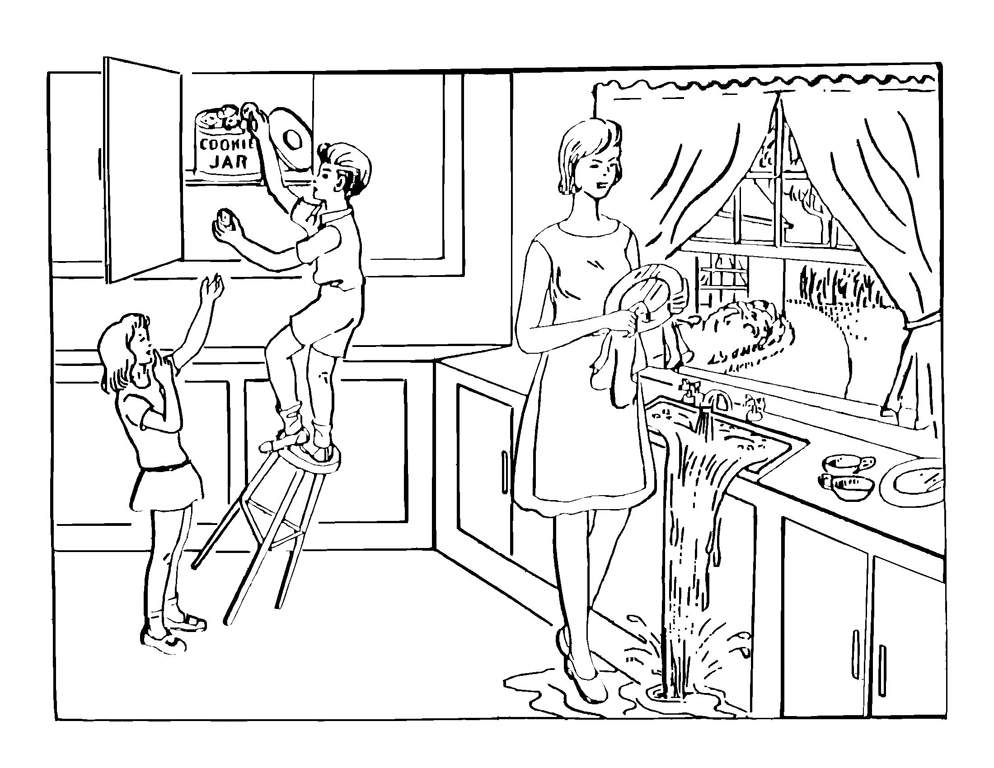
\includegraphics[height=\textwidth, angle=90]{nihss_1.jpg}
\newpage
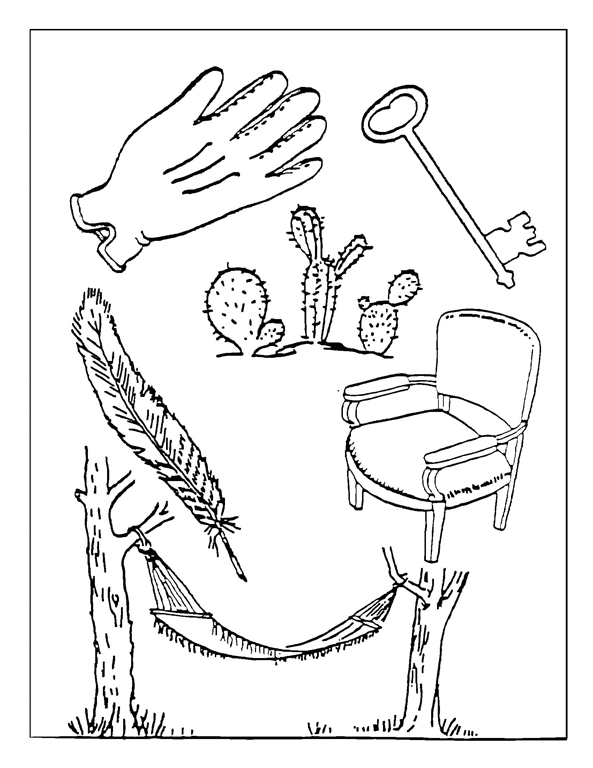
\includegraphics[width=\textwidth]{nihss_3.jpg}
\newpage
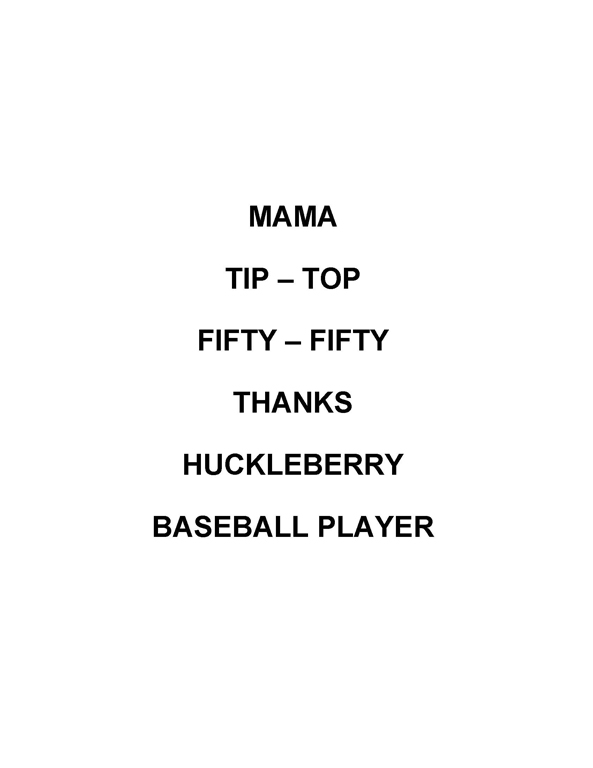
\includegraphics[width=\textwidth]{nihss_4.jpg}
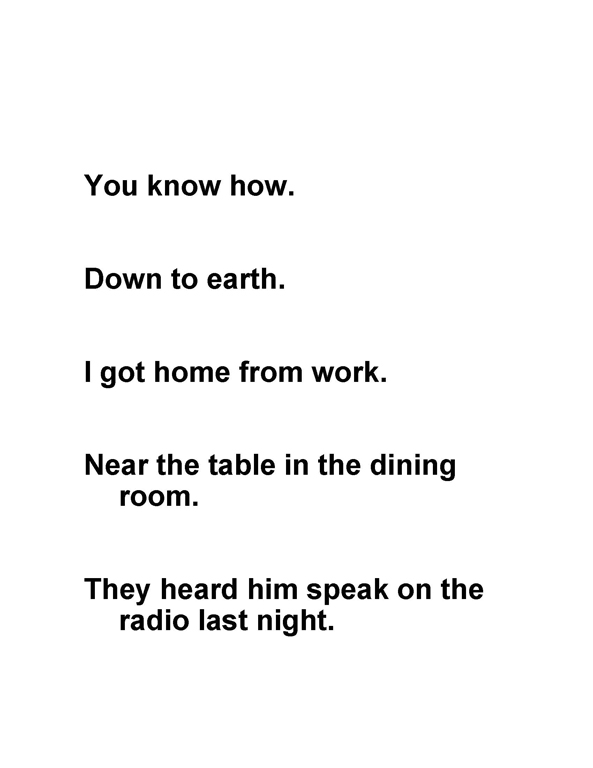
\includegraphics[width=\textwidth]{nihss_2.jpg}

\url{https://stroke.nih.gov/documents/NIH_Stroke_Scale.pdf}
\newpage

\subsection{tPA Criteria}
Inclusion
\begin{itemize}
    \item Diagnosis of ischemic stroke causing measurable neuro deficit
    \item Onset of sx <3 hours before beginning tx
    \item Aged $\gte$18 years
\end{itemize}
Exclusion
\begin{itemize}
    \item Significant head trauma or prior stroke in previous 3 months
    \item Sx suggest SAH
    \item Arterial puncture at noncompressible site in previous 7 days
    \item Hx of previous ICH
    \item Intracranial neoplasm, AVM, or aneurysm
    \item Recent intracranial or intraspinal surgery
    \item BP >185/110
    \item Active internal bleeding
    \item Acute bleeding diathesis
    \item Plt <100k
    \item Heparin within 48h resulting in elevated PTT
    \item Current anticoagulant use with INR >1.7 or PT >15 sec
    \item Current use of direct thrombin inhibitors (Pradaxa) or direct factor Xa inhibitors (Xarelto, Eliquis) with elevated sensitive lab tests
    \item Glucose <50
    \item CT demonstrates multilobular infarction
\end{itemize}
Relative exclusion
\begin{itemize}
    \item Rapidly improving sx
    \item Pregnancy
    \item Seizure at sx onset with postictal state
    \item Major surgery or serious trauma within 14 days
    \item Recent GI hemorrhage or urinary tract hemorrhage within 21 days
    \item Recent MI within 3 months
\end{itemize}
Exclusion for 3-4.5 hours
\begin{itemize}
    \item Age >80 years
    \item NHISS >25
    \item Taking oral anticoagulant regardless of INR
    \item Hx of both DM and prior ischemic stroke
\end{itemize}
tPA dose: 0.9 mg/kg (max 90 mg) over 60 minutes, with 10\% of the dose given as a bolus over 1 minute\\
BP goal: <180/<105. Labetalol 10-20 mg IV x2; or Cardene 5 mg/hr IV, titrate 2.5 mg/hr q5-15min, max 15 mg/hr

\vfill

\tiny{Jauch, et al. Guidelines for the early management of patients with acute ischemic stroke: a guideline for healthcare professionals from the American Heart Association/American Stroke Association. Stroke. 2013 Mar;44(3):870-947. doi: 10.1161/STR.0b013e318284056a. Epub 2013 Jan 31. PubMed PMID: 23370205.}
\newpage
\section{Snellen Chart}


\url{http://www.polk.amedd.army.mil/docs/opt/Eye%20Chart.pdf}

\section{Decision Rules}

\subsection{HEART Score}

\begin{tabularx}{\linewidth}{|X|X|}
\hline
History & 
    \begin{enumerate}
        \item{Slightly suspicious}
        \item{Moderately suspicious}
        \item{Highly suspicious}
    \end{enumerate}
    \\

EKG &
    \begin{enumerate}
        \item{Normal}
        \item{Non-specific repolarization disturbance}
        \item{Significant ST depression}
    \end{enumerate}
    \\
    
Age &
    \begin{enumerate}
        \item{<45}
        \item{45-65}
        \item{>65}
    \end{enumerate}
    \\
    
Risk factors &
    \begin{enumerate}
        \item{No known risk factors}
        \item{1-2 risk factors}
        \item{$\geq$3 risk factors or hx atherosclerotic disease}
    \end{enumerate}
    \\

Initial troponin &
    \begin{enumerate}
        \item{Normal limit}
        \item{1-2x normal limit}
        \item{>2x normal limit}
    \end{enumerate}
    \\
\hline
\end{tabularx}

0-3: 0.9-1.7\% risk of adverse cardiac event. Discharge.\\
4-6: 12-16.6\% risk of adverse cardiac event. Admit.\\
$\geq$7: 50-6\% risk of adverse cardiac event. Early invasive measures.\\

\tiny{Risk factors: HTN, HLD, DM, obesity BMI >30, smoking (current, or cessation <=3 mo), positive family hx (parent or sibilng with CVD before age 65)}\\
\tiny{Atherosclerotic disease: prior MI, PCI/CABG, CVA/TIA, or peripheral artery disease}

\subsection{PERC Rule}
    \begin{itemize}
        \item Age $\gte$50
        \item HR $\gte$100
        \item SaO2 on RA <95%
        \item Unilateral leg swelling
        \item Hemoptysis
        \item Recent surgery or trauma ($\lte$ 4 wks requring GA)
        \item Prior PE or DVT
        \item Hormone use
    \end{itemize}


\section{Imaging}
\subsection{Radiation Doses}

\begin{tabularx}{\linewidth}{|X|X|X|}
\hline
\textbf{Procedure} & \textbf{mSv} & \textbf{Equivalent natural background radiation} \\
\hline
CT A/P & 10 & 3 years  \\
\hline
CT Chest & 7 & 2 years  \\
\hline
CT Head & 2 & 8 months  \\
\hline
XR Upper GI & 6 & 2 years  \\
\hline
CXR & 0.1 & 10 days  \\
\hline
XR Extremity & 0.001 & 3 hours  \\
\hline
\end{tabularx}
\url{https://www.acr.org/~/media/ACR/Documents/PDF/QualitySafety/Radiation-Safety/Dose-Reference-Card.pdf}

\subsection{Ultrasound Imaging Criteria}
\begin{tabularx}{\linewidth}{|X|X|X|X|}
\hline
\textbf{} & \textbf{Windows} & \textbf{Measurements\break Findings}  & \textbf{Notes} \\
\hline
Aorta & Diaphragmatic hiatus (subxyphoid) to bifurcation (umbilicus) & Outside wall to outside wall & Diameter >3 cm and suspected AAA $\rightarrow$ CT  \\
\hline
Cardiac & 
Subxyphoid (9 o'clock)\break 
PLax (4)\break
PSax (8)\break
Apical4c (9)
& 
Pericardial effusion\break
Tamponade\break
Gross cardiac motion\break
EF\%
& - \\
\hline
Kidney and bladder &
Kidney x2\break
Bladder\break
Ureteral jets
& Hydro, size of kidneys & - \\
\hline
Lung and pleura &
Anterior chest\break
Mid-clavicular line just inferior to clavicles\break
Lateral chest\break
Posterior chest\break &
PTX, pleural effusion at bases, B-lines & Perpendicular to ribs \\
\hline
Ocular &
Anterior chamber, Iris, Lens, Posterior chamber &
Fibrinous vitreous bands\break
Retinal detachment (tethered to optic nerve)\break
Posterior vitreous detachment (not tethered)\break
Vitreous hemorrhage\break
Subretinal hemorrhage\break
Lens dislocation\break
Foreign body\break
Globe rupture\break
Retrobulbar hemorrhage\break
Optic nerve edema\break
CRAO\break
Light response\break &
- \\
\hline
\end{tabularx}

\begin{tabularx}{\linewidth}{|X|X|X|X|}
\hline
Pelvic & Uterus, cul-de-sac, ovaries, fallopian tubes & Flow to ovaries & Transvag \= empty bladder \\
\hline
RUQ & GB, CBD (follow neck of GB to portal triad) &
Cholelithiasis\break
Cholecystitis (AGBW >3mm, pericholecystic fluid, sonographic Murphy's, GB diameter >5 cm)\break
CBD dilation >3mm (+1 for each decade) &
CBD inner-to-inner \\
\hline
MSK & Soft tissue, bones, joint effusion, tendons/ligaments & Cellulitis, abscess, FB, deep space infections, joint effusions, arthrocentesis, fractures, tendon/ligament lacerations and ruptures, tenosynovitis & - \\
\hline
DVT & 
Common femoral vein (CFV)\break
Saphenofemoral junction (SFJ)\break
Deep femoral vein\break
Popliteal vein\break
Trifurcation\break &
- & \raisebox{-1\height}{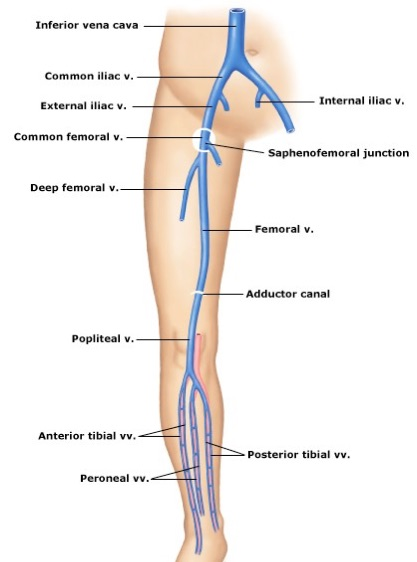
\includegraphics[width=\linewidth]{LE_veins.jpg}} \\
\hline
\end{tabularx}
\url{https://www.acep.org/Clinical---Practice-Management/} \url{Emergency-Ultrasound-Imaging-Criteria-Compendium/}
Image: \url{http://imbus.anwresidency.com/txtbook/18_vte.html}

\section{Pediatrics}

\url{https://i.pinimg.com/originals/7e/23/4d/7e234dc68b4ec37246f64eef79857c10.jpg}
\url{http://s3.amazonaws.com/media.matthewsbooks.com/images/GROUP002/1890495344.jpg}

DISEASE BY AGE

\newpage

\section{STEMI}
\subsection{STEMI Equivalents}
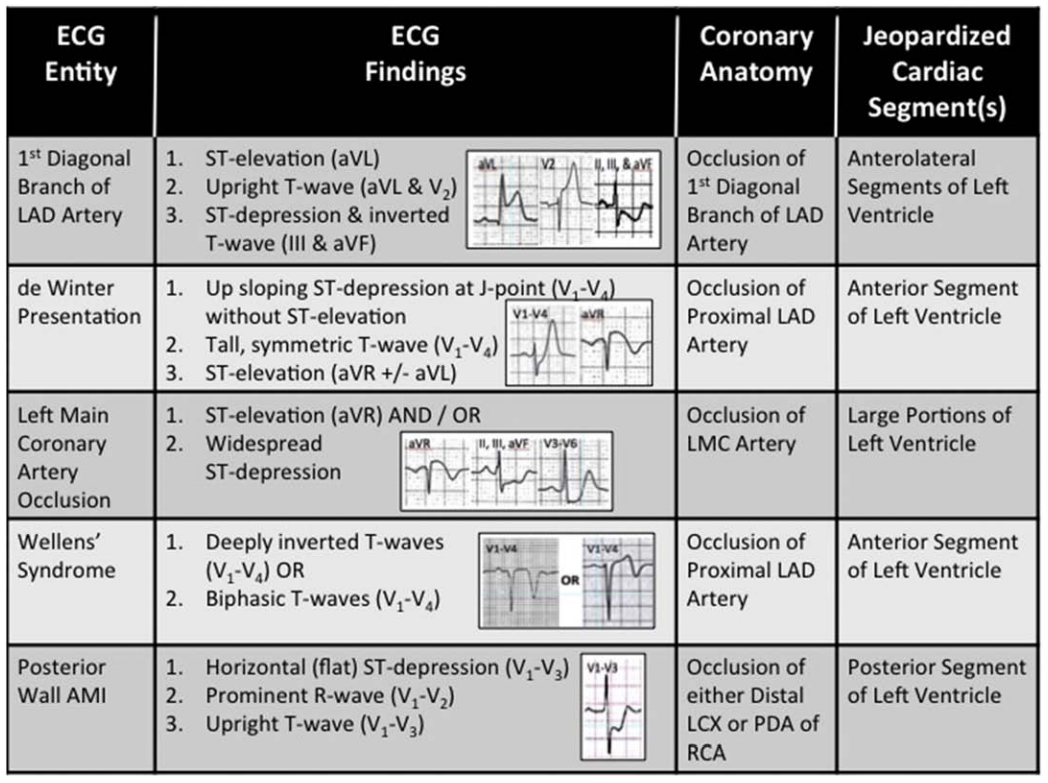
\includegraphics[height=\textwidth, angle=90]{5_ecgs.png}
Activate cath lab for all except Wellens (interventional cardiology consult)\break

\tiny{Macias M, et al. The electrocardiogram in the ACS
patient: high-risk electrocardiographic presentations lacking anatomically oriented ST-segment elevation. Am J Emerg Med. 2016 Mar;34(3):611-7. doi:10.1016/j.ajem.2015.11.047. Epub 2015 Dec 2. Review. PubMed PMID: 26742458.}
\subsection{Right}
RV infarction is seen in 40\% of inferior STEMIs.\break
85\% of inferior STEMI are due to RCA occlusion. The RCA supplies the RV, and usually also supplies the inferior wall. (Except in patients whose circumflex (branch of LCA) supplies the inferior wall.)
\begin{itemize}
    \item ST elevation in V1. ST elevation in lead III > II.
    \item Give IVF and avoid NTG.
    \item Get right-sided EKG.
\end{itemize}
\subsection{Posterior}
Posterior infarction is suggested by V1-V3 showing
\begin{itemize}
    \item ST depression
    \item Tall, broad R waves
    \item Upright T waves
    \item Dominant R wave (R/S ratio > 1) in V2
\end{itemize}

\section{Orthopedics}
\subsection{Exam}
\begin{tabularx}{\linewidth}{|X|X|}
\hline
Shoulder & 
    \begin{itemize}[leftmargin=*]
        \item[] Flexion/Extension
        \item[] Internal/External Rotation
        \item[] Apley scratch test (touch opposite scapula)
        \item[] Empty can test
        \item[] Median/ulnar/radial/axillary sens
        \item[] Radial pulse 2+
        \item[] DTR bicep/tricep 2+
    \end{itemize}\\
\hline
Elbow & 
    \begin{itemize}[leftmargin=*]
        \item[] ROM
        \item[] Supination/pronation
        \item[] Stability
        \item[] No varus or valgus laxity
        \item[] Lateral epicondyle tenderness
        \item[] Sensation/pulse/DTRs
    \end{itemize}\\
\hline
Wrist/Hand & 
    \begin{itemize}[leftmargin=*]
        \item[] Nontender, no effusion
        \item[] Wrist flexion/extension
        \item[] Radial/ulnar deviation
        \item[] Able to A-OK, hook horns, cross fingers, thumbs up bilaterally
        \item[] No wrist instability
        \item[] Tinel's negative at the carpal tunnel
        \item[] MCP, PIP, DIP extension and flexion of each finger
        \item[] Sensation/pulse/DTRs
    \end{itemize}\\
\hline
Hip & 
    \begin{itemize}[leftmargin=*]
        \item[] Flx/ext/ad/ab
        \item[] L2 iliopsoas/mid anterior thigh sensation
        \item[] L3 quad/distal anterior thigh sensation
        \item[] L4 tibialis anterior/patellar reflex/medial ankle sensation
        \item[] L5 EHL/dorsal foot sensation
        \item[] S1 peroneals/Achilles reflex/lateral ankle sensation
        \item[] Patellar and Achilles DTRs 2+
    \end{itemize}\\
\hline
Knee & 
    \begin{itemize}[leftmargin=*]
        \item[] ROM
        \item[] Stability: Anterior drawer, Lachman, Posterior Drawer, Varus, Valgus
        \item[] EHL, tibialis anterior, plantar flexion 5/5
    \end{itemize}\\
\hline
Ankle/Foot & 
    \begin{itemize}[leftmargin=*]
        \item[] Dorsiflexion/plantarflexion
        \item[] Talar tilt
    \end{itemize}\\
\hline
\end{tabularx}

\subsection{Ottawa rules}
\subsubsection{Ottowa ankle rule}
Ankle XR needed if
    \begin{itemize}
        \item Pain near the maleoli AND
        \item Inability to bear weight immediately and in the ED (4 steps) OR
        \item Tenderness at posterior edge or tip of lateral malleolus OR
        \item Tenderness at posterior edge or tip of medial malleolus
    \end{itemize}
Foot XR needed if
    \begin{itemize}
        \item Pain in the midfoot AND
        \item Inability to bear weight both immediately and in the ED (4 steps) OR
        \item Tenderness at the navicular OR
        \item Tenderness at the base of the 5th metatarsal
    \end{itemize}
Ages 6-55, blunt trauma only

\newpage

\section{Toxicology}
\subsection{Methemoglobinemia and cyanide}
\subsubsection{Methemoglobinemia}
Hb \xrightarrow[]{\begin{subarray}{c} TMP-SMX \\ dapsone \\ benzocaine \\ Reglan \\ nitrates \end{subarray}} Met-Hb

\vfill

Hb \xleftarrow[]{methylene blue} Met-Hb

\vfill

\subsubsection{Cyanide}
CN \xrightarrow[]{hydroxycobalamin} B12 (cyanocobalamin)

\vfill

Hb \xrightarrow[]{\begin{subarray}{c} amyl nitrite \\ sodium nitrite \end{subarray}} Met-Hb \xrightarrow[]{CN} CN-Met-Hb \xrightarrow[]{Na-thiosulfate} Na-thiocyanate \\ (renally excreted)

\vfill


\end{document}
